\documentclass{extbook}[14pt]
\usepackage{multicol, enumerate, enumitem, hyperref, color, soul, setspace, parskip, fancyhdr, amssymb, amsthm, amsmath, bbm, latexsym, units, mathtools}
\everymath{\displaystyle}
\usepackage[headsep=0.5cm,headheight=0cm, left=1 in,right= 1 in,top= 1 in,bottom= 1 in]{geometry}
\pagestyle{fancy}
\lhead{}
\chead{Answer Key for Module\,12M\,-\,Solving\,Word\,Problems Version A}
\rhead{}
\lfoot{Summer\,C\,2020}
\cfoot{}
\rfoot{}
\begin{document}
\textbf{This key should allow you to understand why you choose the option you did (beyond just getting a question right or wrong). \href{https://xronos.clas.ufl.edu/mac1105spring2020/courseDescriptionAndMisc/Exams/LearningFromResults}{More instructions on how to use this key can be found here}.}

\textbf{If you have a suggestion to make the keys better, \href{https://forms.gle/CZkbZmPbC9XALEE88}{please fill out the short survey here}.}

\textit{Note: This key is auto-generated and may contain issues and/or errors. The keys are reviewed after each exam to ensure grading is done accurately. If there are issues (like duplicate options), they are noted in the offline gradebook. The keys are a work-in-progress to give students as many resources to improve as possible.}

\rule{\textwidth}{0.4pt}

1. Solve the modeling problem below, if possible.
A new virus is spreading throughout the world. There were initially 7 many cases reported, but the number of confirmed cases has quadrupled every 5 days. How long will it be until there are at least 1000000 confirmed cases? 
The solution is $ \text{About } 43 \text{ days} $ 

\begin{enumerate}[label=\Alph*.] 
\item $ \text{About } 21 \text{ days} $ 

 You modeled the situation correctly but did not apply the properties of log correctly. 
\item $ \text{About } 60 \text{ days} $ 

 You modeled the situation with $e$ as the base, but solved correctly otherwise. 
\item $ \text{About } 24 \text{ days} $ 

 You modeled the situation with $e$ as the base and did not apply the properties of log correctly. 
\item $ \text{About } 43 \text{ days} $ 

 * This is the correct option. 
\item $ \text{There is not enough information to solve the problem.} $ 

 If you chose this option, please contact the coordinator to discuss why you think this is the case. 
\end{enumerate} 
 
\textbf{General Comment:} \textbf{General Comments:} Set up the model the same as in Module 11M. Then, plug in 1000000 and solve for $d$ in your model. 

-----------------------------------------------

2. For the scenario below, find the variation constant $k$ of the model (if possible).
In an alternative galaxy, the quartic of the time, $T$ (Earth years), required for a planet to orbit Sun $\chi$ increases as the cube of the distance, $d$ (AUs), that the planet is from Sun $\chi$ increases. For example, when Ea's average distance from Sun $\chi$ is 4, it takes 92 Earth days to complete an orbit. 
The solution is $ k = 1119364.000 $ 

\begin{enumerate}[label=\Alph*.] 
\item $ k = 1119364.000 $ 

 * This is the correct option corresponding to the model $T^{4} = k d^{3}$. 
\item $ k = 1.951 $ 

 This corresponds to the model $T^{1/4} = k d^{1/3}$. 
\item $ k = 4.028 $ 

 This copies the constant used in the homework. 
\item $ k = 4584914944.000 $ 

 This corresponds to the model $T^{4} = \frac{k}{d^{3}}$. 
\item $ \text{Unable to compute the constant based on the information given.} $ 

 This corresponds to believing you cannot determine the type of model from the information given. 
\end{enumerate} 
 
\textbf{General Comment:} \textbf{General comments:} since $T$ increases proportionally as $d$ increases, we know this is a direct variation model. 

-----------------------------------------------

3. Determine the appropriate model for the graph of points below.
\begin{center} 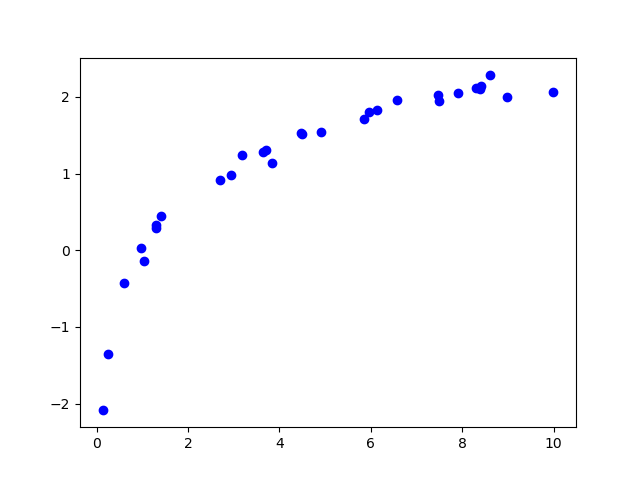
\includegraphics[width=0.3\textwidth]{../Figures/identifyModelGraph12A.png} \end{center} 

The solution is $ \text{Logarithmic model} $ 

\begin{enumerate}[label=\Alph*.] 
\item $ \text{Exponential model} $ 

 For this to be the correct option, we want an extremely slow change early, then a rapid change later. 
\item $ \text{Logarithmic model} $ 

 For this to be the correct option, we want a rapid change early, then an extremely slow change later. 
\item $ \text{Linear model} $ 

 For this to be the correct option, we need to see a mostly straight line of points. 
\item $ \text{Non-linear Power model} $ 

 For this to be the correct option, we need to see a polynomial or rational shape. 
\item $ \text{None of the above} $ 

 For this to be the correct option, we want to see no pattern in the points. 
\end{enumerate} 
 
\textbf{General Comment:} \textbf{General comments:} This question is testing if you can associate the models with their graphical representation. If you are having trouble, go back to the corresponding Core module to learn about the specific function you are having trouble recognizing. 

-----------------------------------------------

4. For the scenario below, use the model for the volume of a cylinder as $V = \pi r^2 h$.
Pringles wants to add 48 \text{percent} more chips to their cylinder cans and minimize the design change of their cans. They've decided that the best way to minimize the design change is to increase the radius and height by the same percentage. What should this increase be? 
The solution is $ \text{About } 14 \text{ percent} $ 

\begin{enumerate}[label=\Alph*.] 
\item $ \text{About } 24 \text{ percent} $ 

 This corresponds to treating both radius and height as equal contributors and not solving correctly. 
\item $ \text{About } 14 \text{ percent} $ 

 * This is the correct option. 
\item $ \text{About } 22 \text{ percent} $ 

 This corresponds to solving correctly but treating both radius and height as equal contributors to the volume. 
\item $ \text{About } 4 \text{ percent} $ 

 This corresponds to not solving for the increase properly. 
\item $ \text{None of the above} $ 

 If you chose this, please contact the coordinator to discus how you solved the problem. 
\end{enumerate} 
 
\textbf{General Comment:} \textbf{General Comments:} Remember that when plugging the increases of values in, you need to treat it as that percentage above 100. For example, a 5 percent increase means 105 percent. 

-----------------------------------------------

0. Solve the modeling problem below, if possible.
In CHM2045L, Brittany created a 19 liter 15 percent solution of chemical $\chi$ using two different solution percentages of chemical $\chi$. When she went to write her lab report, she realized she forgot to write the amount of each solution she used! If she remembers she used 13 percent and 33 percent solutions, what was the amount she used of the 33 percent solution? 
The solution is $ 1.90 $ 

\begin{enumerate}[label=\Alph*.] 
\item $ 1.90 $ 

 *This is the correct option. 
\item $ 1.15 $ 

 This was a random value. If this was not a guess, contact the coordinator to talk about how you got this value. 
\item $ 17.10 $ 

 This is the concentration of 13 percent solution. 
\item $ 9.50 $ 

 This would be correct if Brittany used equal parts of each solution. 
\item $ \text{There is not enough information to solve the problem.} $ 

 You may have chose this if you thought you needed to know how much of the second solution was used in the problem. Remember that the total minus the first solution would give you the second amount used. 
\end{enumerate} 
 
\textbf{General Comment:} \textbf{General Comments:} Build the model exactly as you did in Module 9M. Then, solve for the volume you are looking for. 

-----------------------------------------------


\end{document}

